\newpage
\chapter{MIDAS}
\label{chap:mc}
\workTodo{In diesem Kapitel werden grundlegende Themen behandelt, die im Rahmen des Forschungsprojekts zum Verst�ndnis der Ausrei�er-Erkennung in Graphen gedient haben.}

Erst erkl�ren wie der MIDAS funktioniert. Und zum Laufen gebracht mit Graphen �ber die Zeit ENRON \& DARPA. Im Anschluss auf Zeitreihendaten angewendet.

\section{Grundlagen}
\label{sec:mc-gl}
\workTodo{Einf�hrung in den Algorithmus}


\subsection{Count-min Sketch}
\label{sec:mc-gl-cms}

\subsubsection{Einf�hrung}
\label{sec:mc-gl-cms-in}

\workTodo{Stichworte sammeln}

\section{Ergebnisse Ausrei�ererkennung in Zeitreihen}
uiebwiebdciqbewd
\label{sec:resultsOTs}

\begin{figure}[h]
	\centering
	\subfloat{
		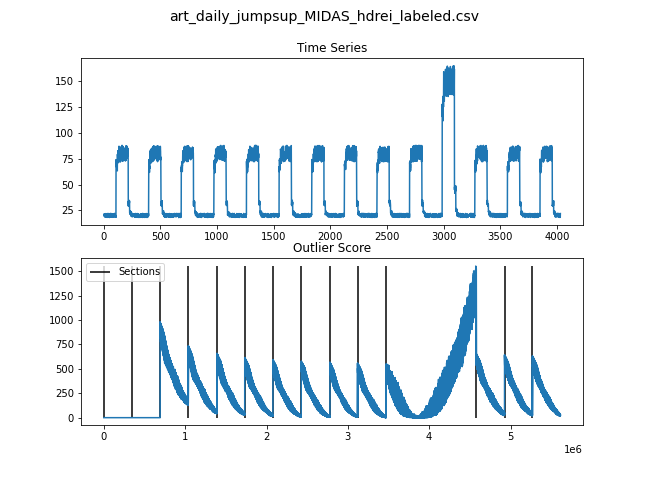
\includegraphics[width=0.5\textwidth]{fig/resultsMidasTS/art_daily_jumpsup_MIDAS_hdrei_labeled_result.png}}
	\subfloat{
		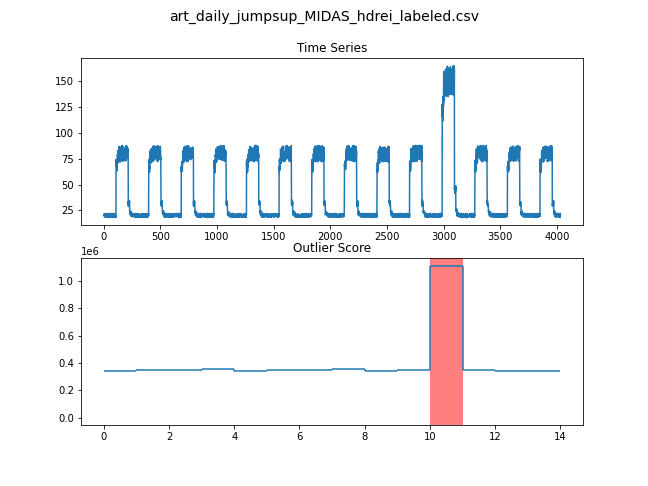
\includegraphics[width=0.5\textwidth]{fig/resultsMidasTS/result_without_midas.png}}
	\caption{Vergelich Perculation Algorithmus mit Sliding Window Verfahren und ohne Sliding Window Verfahren}
	\label{img:midasTSresults}
\end{figure}

